\documentclass[11pt, oneside]{article} 
\usepackage{geometry}
\geometry{letterpaper} 
\usepackage{graphicx}
	
\usepackage{amssymb}
\usepackage{amsmath}
\usepackage{parskip}
\usepackage{color}
\usepackage{hyperref}

\graphicspath{{/Users/telliott_admin/Tex/png/}}
% \begin{center} 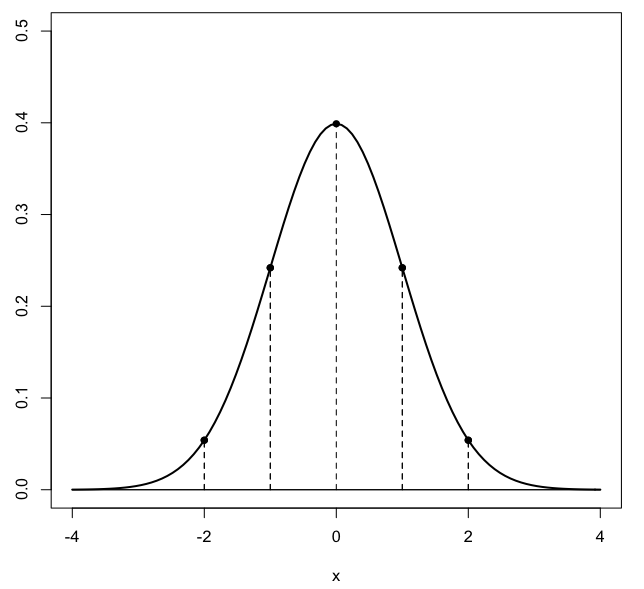
\includegraphics [scale=0.4] {gauss3.png} \end{center}

\title{Circular segment}
\date{}

\begin{document}
\maketitle
\Large

I found a hard geometry problem on the web
\begin{center} 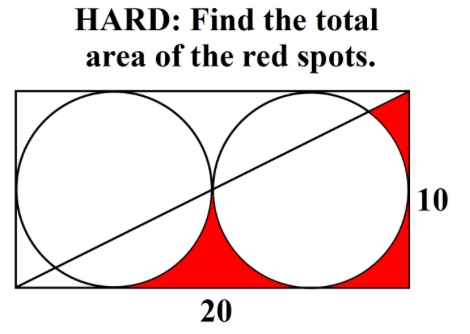
\includegraphics [scale=0.4] {circ_seg_prob.png} \end{center}
We know it's hard because it says so!

The area of a red corner is pretty easy, $4$ of them together are equal to the difference between the square with side length $10$ and the circle of radius $5$
\[ 4q = 100 - \pi 5^2 \approx 21.46 \]

The problem is the upper right-hand corner.
\begin{center} 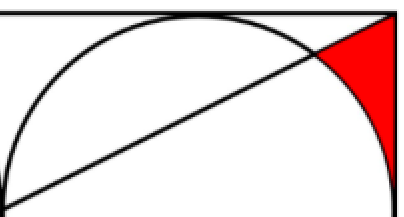
\includegraphics [scale=0.25] {circ_seg_prob2.png} \end{center}
One way to solve that is to view this as two triangles.  The upper one contains a circular segment, if we knew that we could get the arc-like segment of the lower triangle and then the red part by subtraction.

From the geometry we know that these two smaller) right triangles have sides $5$ and $10$. 

The smaller angle, call it $\phi$, is  $\phi = \tan^{-1} 1/2 \approx 0.4636$ radians or about $26.565$ degrees.

To proceed in this way we also need either the length of the chord $a$ or the height of the segment $h$ or the angle cut out from the center of the circle by the segment, $\theta$.
\begin{center} 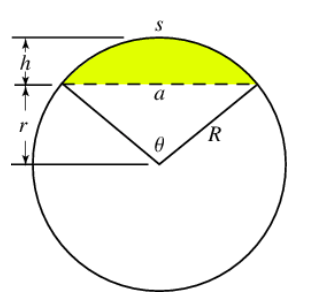
\includegraphics [scale=0.5] {circ_seg.png} \end{center}

\url{http://mathworld.wolfram.com/CircularSegment.html}

\subsection*{if we had $h$ or $r$ or $\theta$}
We need both $\theta$ and $a$

If we have $h$, we get $r$ as $R - h$.  

If we have $r$, we get $\theta/2 = \cos^{-1} r/R$.

If we have $\theta$, we get $r = R \cos \theta/2$.  We also get $a/2 = R \sin \theta/2$.

The area of the whole wedge of the unit circle cut out with angle $\theta$ is
\[ A = \frac{\theta}{2\pi} \ \pi R^2 \]  
The area of the rest of the wedge is the area of the triangle with base $a$ and sides $R$.  The height of that triangle is $\sqrt{R^2 - (a/2)^2}$ and its area is
\[ A_{\text{tri}} = \frac{1}{2} \ a \sqrt{R^2 - (a/2)^2} \]

Given $h$ by itself, another approach would be to integrate the unit circle from $R-h \rightarrow R$.

\subsection*{$a$ by itself}
Unfortunately, $h$, $r$ and the angle $\theta$ all look problematic.

How about $a$, the length of the chord?
\begin{center} 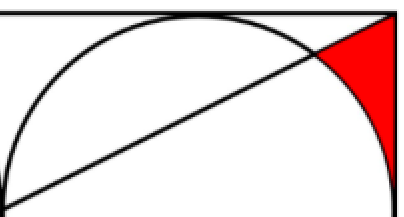
\includegraphics [scale=0.25] {circ_seg_prob2.png} \end{center}

Consider this half-circle to be part of a unit circle with the origin placed as usual.  What is the equation of the line?  It has slope 0.5 and $y$-intercept 0.5
\[ y = 0.5 x + 0.5 \]
Since $x^2 + y^2 = 1$
\[ \sqrt{1 - x^2} = 0.5 x + 0.5 \]
\[ 2 \sqrt{1 - x^2} = x + 1 \]
\[ (4 - 4x^2) = (x + 1)^2 \]
\[ 5x^2 + 2x - 3 = 0 \]
\[ x = \frac{-2 \pm \sqrt{4 + 60}}{10} \]
\[ = -1, 0.6 \]

That worked out nicely!  The meaning of $-1$ is obvious, and $0.6$ is what we seek.  The corresponding $y$ is also nice
\[ y = 0.5 x + 0.5 = 0.3 + 0.5 = 0.8 \]

The two intersections with the circle form the hypotenuse of a right triangle with base equal to $1.6$ and height equal to $0.8$ 
\[ \sqrt{1.6^2 + 0.8^2} = \sqrt{3.2} \approx 1.7889 \]

\subsection*{going backward}
We're not there yet, the Wolfram article again gives the geometry.
\begin{center} 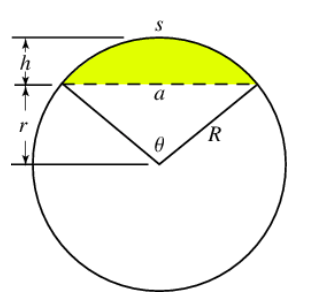
\includegraphics [scale=0.5] {circ_seg.png} \end{center}

Now we've determined the chord $a$, $1.7889$ for the unit circle and $5$ times that for our dimensions, and the half-length of the chord ($4.472$), we obtain 
\[ r^2 = R^2 - (\frac{a}{2})^2 \]
$4.472$ is the square root of $20$!  There is obviously some easy geometry that I'm missing here!  So

\[ r^2 = 25 - 20 = 5 \]
\[ r = \sqrt{5} \approx 2.236 \]

As we said before, from $r$ we can find $\theta$ and thence the area of the sector, and then subtract the area of the triangle with height $r$ and base $a$.

Alternatively we can get 
\[ h = R - r = 5 - \sqrt{5} \]
and then integrate
\[ \int_{R-h}^R \sqrt{R^2 - x^2} \ dx \]
\[= \frac{1}{2} \ [ \ \sin^{-1} x + x \sqrt{1 - x^2} \ ] \ \bigg |_{R-h}^R \]

That's all quite a mess!

\subsection*{polar equation}

I had two better ideas.  

The first was to look again at
\begin{center} 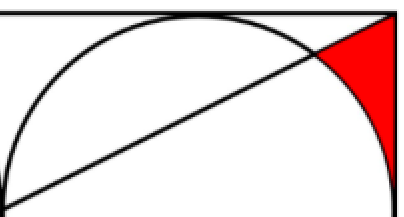
\includegraphics [scale=0.25] {circ_seg_prob2.png} \end{center}

What if we could get the area of the lower triangle minus the red part?

If we set up a circle of radius $a$ with its left edge at the origin, the equation of that circle in polar coordinates is
\[ r = 2 a \cos \phi \]

For example, radius $a = 1$ gives
\[ \phi = 0, \ \ \ \ r = 2 \]
\[ \phi = \frac{\pi}{4}, \ \ \ \ r = \sqrt{2} \]
\[ \phi= \frac{\pi}{2}, \ \ \ \ r = 0 \]
The arc that we're seeing is $\phi = 0 \rightarrow \frac{\pi}{2}$

You don't believe me that this equation is correct?  For $a = 1$
\[ r = 2 \cos \phi \]
but
\[ \cos \phi = rx \]
\[ r^2 = 2x \]
\[ = x^2 + y^2  \]
We obtain
\[ x^2 + y^2 = 2x \]
\[ x^2 - 2x + y^2 = 0 \]
Complete the square and add the same term on the right
\[ (x - 1)^2 + y^2 = 1 \]
This is indeed a unit circle with origin at $(1,0)$.

\subsection*{polar area}

The area is made up of many small wedges with angle $\phi$, and $r = f(\phi)$.  The wedges are approximately triangles with area $1/2 \cdot r \cdot r \ d \theta$.  So the total area is

\[ A = \int \frac{1}{2} \ [ \ f(\theta) \ ]^2 \ d \theta \]

\[ = \frac{1}{2} a^2 \int \cos^2 \theta \ d \theta\]
\[ = \frac{1}{2} a^2 \ [ \ \frac{1}{2} (\theta + \sin \theta \cos \theta) \ ] \ \bigg |_0^{\phi} \]
At the lower bound, this is zero so
\[ A = \frac{1}{4} a^2 \  (\phi + \sin \phi \cos \phi) \] 

We can get $\phi$ from the diagram.  By similar triangles, 
\[ \tan \phi = 0.5 \]
\[ \phi = 0.4637\]

Also
\[ \sin \phi = \frac{1}{\sqrt{5}} \]
\[ \cos \phi = \frac{2}{\sqrt{5}} \]
\[ \sin \phi \cos \phi = \frac{1}{\sqrt{5}} \cdot \frac{2}{\sqrt{5}} \]
\[ = \frac{2}{5} \]

\[ A = 25 (0.4637 + \frac{2}{5}) =  \]
We must subtract this from the area of the triangle, which is $5 \cdot 10 / 2$ = 25.

The answer is $0.136 \times 25$, which doesn't look unreasonable.

\subsection*{another idea}
The other idea was to look again at
\begin{center} 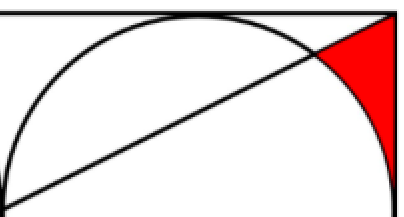
\includegraphics [scale=0.25] {circ_seg_prob2.png} \end{center}

Starting from the center of the circle corresponding to this half-circle, draw the radius out to the left.  This forms the angle that we called $\phi$ above.

Now draw the other radius up to where the red stuff touches the perimeter of the circle.

Belatedly, I realize that I've just drawn an isosceles triangle because of the two radii.  The large angle of this triangle is $\theta$!

\[ \theta + 2 * \phi = 180 \]
\[ \theta = 126.87 \]

\begin{center} 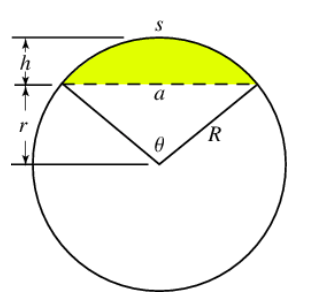
\includegraphics [scale=0.5] {circ_seg.png} \end{center}

Remember what we said before:  if we have $\theta$, we get $r = R \cos \theta/2$.  We also get $a/2 = R \sin \theta/2$.
\[ r = 5 \cos \theta/2 = 2.236 \]
\[ a = 10 \sin \theta/2 = 8.944 \]

The angle of the triangle with base $a$ is exactly $ar/2 = 10.000000$.

There is obviously some beautiful geometry that I'm missing.

To finish this off we need the area of the sector, and subtract the above area from it.

Or else...
\begin{center} 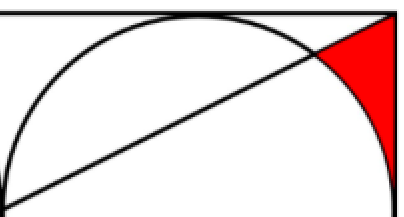
\includegraphics [scale=0.25] {circ_seg_prob2.png} \end{center}

Calculate the area of a sector of the circle with angle $2 \phi$.  Add that to area of $10$ that we got above and subtract that sum from the triangle $25$.

\[ \phi = tan^{-1} 0.5 = 0.463 \text{rad} \]

The area of the sector is $2 \phi/2 \pi = \phi / \pi = 0.14758$ times the area of the circle $\pi 5^2$.  

\[ 25 - 10 - (\phi * 25) = 3.4088 \]

Some mistake.



\end{document}